
\chapter{Q-Learning}

% https://blog.csdn.net/qq_30615903/article/details/80739243
% https://www.freecodecamp.org/news/an-introduction-to-q-learning-reinforcement-learning-14ac0b4493cc/

% 视频 https://v.youku.com/v_show/id_XMTk2NzM1Mjk5Mg==.html

% 发现了很多RL资料搬砖过来,刚入门的可以用得上

% David Silver 博士的 UCL 公开课:http://www0.cs.ucl.ac.uk/staff/d.silver/web/Teaching.html
% DeepMind 和 UCL 的DL、RL课程:https://www.youtube.com/playlist?list=PLqYmG7hTraZDNJre23vqCGIVpfZ_K2RZs
% Sergey Levine 的DRL课程:http://rail.eecs.berkeley.edu/deeprlcourse/
% OpenAI 的 Spinning Up in Deep RL:https://blog.openai.com/spinning-up-in-deep-rl/
% 关于深度强化学习良心paper:https://arxiv.org/abs/1810.06339

In reinforcement learning, the state-value function is usually denoted by $v$, 
while the action-value function is denoted by $q$.
The $q$ in $q$-learning is in fact refer to the action-value function. 
$Q$-learning is at the heart of all reinforcement learning algorithms.

\section{What is $Q$-Learning ?}

$Q$-Learning is a Reinforcement learning policy that will find the next best action, 
given a current state. It chooses this action at random and aims to maximize the reward.

\begin{figure}[!htb]
\centering
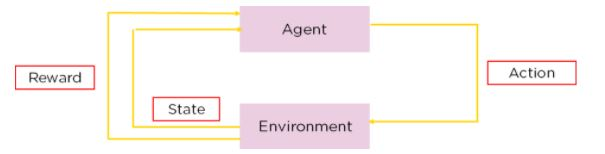
\includegraphics[scale=0.618]{pix/q_learning/3-components-q.jpg}
\caption{Components of Q-Learning}
%\label{fig:label}
\end{figure}



\subsection{Q-Learning — a simplistic overview}

Let's say that a robot has to cross a maze and reach the end point. There are mines, 
and the robot can only move one tile at a time. If the robot steps onto a mine, the 
robot is dead. The robot has to reach the end point in the shortest time possible.

The scoring/reward system is as below:
\begin{itemize}
%\setlength{\itemsep}{0pt}
%\setlength{\parsep}{0pt}
\setlength{\parskip}{0pt}
\item[1.]
The robot loses 1 point at each step. This is done so that the robot takes the 
shortest path and reaches the goal as fast as possible.

\item[2.]
If the robot steps on a mine, the point loss is 100 and the game ends.

\item[3.]
If the robot gets power \textcolor{magenta}{⚡️}, it gains 1 point.

\item[4.]
If the robot reaches the end goal, the robot gets 100 points.
\end{itemize}

Now, the obvious question is: {\bf How do we train a robot to reach the end goal 
with the shortest path without stepping on a mine?}

\begin{figure}[!htb]
\centering
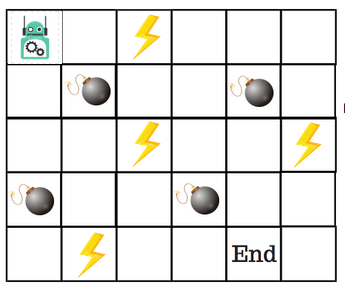
\includegraphics[scale=0.618]{pix/q_learning/q_robot_maze.png}
\caption{Maze}
%\label{fig:label}
\end{figure}
So, how do we solve this?


\subsection{Introducing the Q-Table}

\begin{tabular}{|c||c|c|}
\hline
$Q$-Table	& $a_1$	& $a_2$ \\
\hline
$s_1$	& $q(s_1,a_1)$	& $q(s_1,a_2)$ \\
\hline
$s_2$	& $q(s_2,a_1)$	& $q(s_2,a_2)$ \\
\hline
$s_3$	& $q(s_3,a_1)$	& $q(s_3,a_2)$ \\
\hline
\end{tabular}\;

\vspace

Q-Table is just a fancy name for a simple lookup table where we calculate the 
maximum expected future rewards for action at each state. Basically, this table 
will guide us to the best action at each state.

\begin{figure}[!htb]
\centering
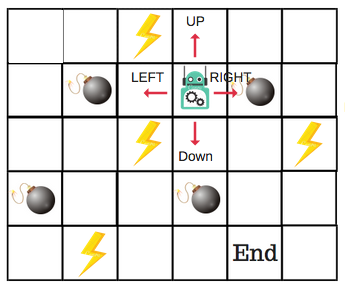
\includegraphics[scale=0.618]{pix/q_learning/q_robot_maze_actions.png}
\caption{Maze: actions}
%\label{fig:label}
\end{figure}
There will be four numbers of actions at each non-edge tile. When a robot is at a 
state it can either move up or down or right or left.

So, let's model this environment in our Q-Table.

In the Q-Table, the columns are the actions and the rows are the states.

\begin{figure}[!htb]
\centering
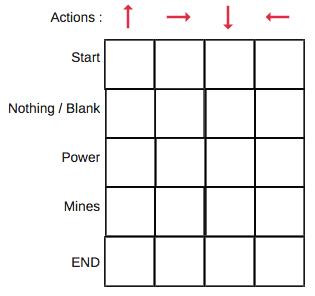
\includegraphics[scale=0.618]{pix/q_learning/q_robot_maze_table.png}
\caption{Maze: q-table}
%\label{fig:label}
\end{figure}

Each Q-table score will be the maximum expected future reward that the robot will 
get if it takes that action at that state. This is an iterative process, as we need 
to improve the Q-Table at each iteration.

But the questions are:

\begin{itemize}
%\setlength{\itemsep}{0pt}
%\setlength{\parsep}{0pt}
\setlength{\parskip}{0pt}
\item[-]
How do we calculate the values of the Q-table?
\item[-]
Are the values available or predefined?
\end{itemize}

To learn each value of the Q-table, we use the Q-Learning algorithm.


\section{Mathematics behind the Q-Learning algorithm}

\subsection{Q-function}

The Q-function uses the Bellman equation and takes two inputs: state (s) and action (a).

\begin{figure}[!htb]
\centering
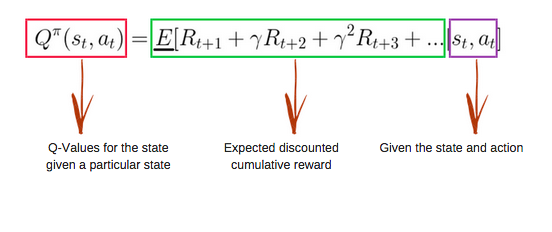
\includegraphics[scale=0.618]{pix/q_learning/q_function.png}
\caption{Maze: q-function}
%\label{fig:label}
\end{figure}

Using the above function, we get the values of Q for the cells in the table.

When we start, all the values in the Q-table are zeros.

There is an iterative process of updating the values. As we start to explore the 
environment, the Q-function gives us better and better approximations by continuously 
updating the Q-values in the table.

Now, let's understand how the updating takes place.


\subsection{Introducing the $Q$-learning algorithm process}

\begin{figure}[!htb]
\centering
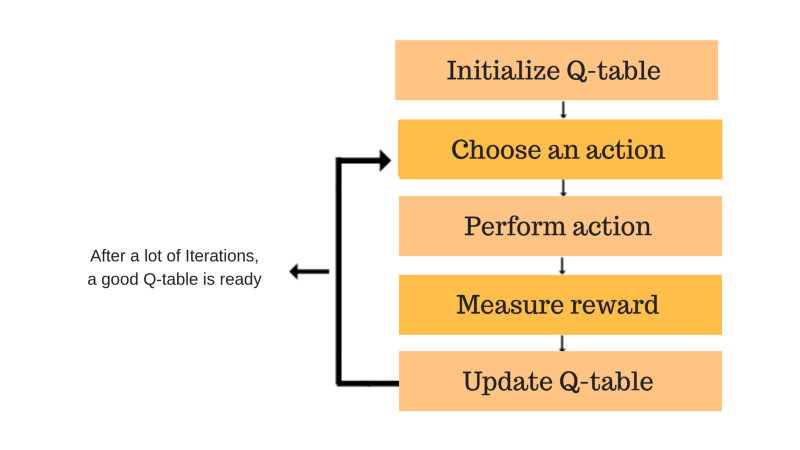
\includegraphics[scale=0.4]{pix/q_learning/q_learning_algorithm_process.png}
\caption{Maze: algorithm process}
%\label{fig:label}
\end{figure}
Each of the colored boxes is one step. Let's understand each of these steps in detail.


\subsubsection{Step 1: initialize the $Q$-Table}
We will first build a $Q$-table. There are $n$ columns, where $n=$ number of actions. 
There are m rows, where m= number of states. We will initialise the values at 0.

\begin{figure}[!htb]
\centering
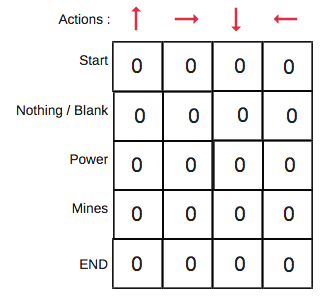
\includegraphics[scale=0.5]{pix/q_learning/q_robot_maze_table_init.png}
\caption{Maze: q-table initialization}
%\label{fig:label}
\end{figure}
In our robot example, we have four actions ($a=4$) and five states ($s=5$). So we will 
build a table with four columns and five rows.


\subsubsection{Steps 2 and 3: choose and perform an action}

This combination of steps is done for an undefined amount of time. This means that 
this step runs until the time we stop the training, or the training loop stops as 
defined in the code.

We will choose an action ($a$) in the state ($s$) based on the $Q$-Table. But, as 
mentioned earlier, when the episode initially starts, every $Q$-value is $0$.

So now the concept of exploration and exploitation trade-off comes into play. This 
chapter has more details.

We'll use something called the {\bf epsilon greedy strategy}.

In the beginning, the epsilon rates will be higher. The robot will explore the 
environment and randomly choose actions. The logic behind this is that the robot 
does not know anything about the environment.

As the robot explores the environment, the epsilon rate decreases and the robot 
starts to exploit the environment.

During the process of exploration, the robot progressively becomes more confident in 
estimating the $Q$-values.

For the robot example, there are four actions to choose from: up, down, left, and 
right. We are starting the training now — our robot knows nothing about the 
environment. So the robot chooses a random action, say right.

\begin{figure}[!htb]
\centering
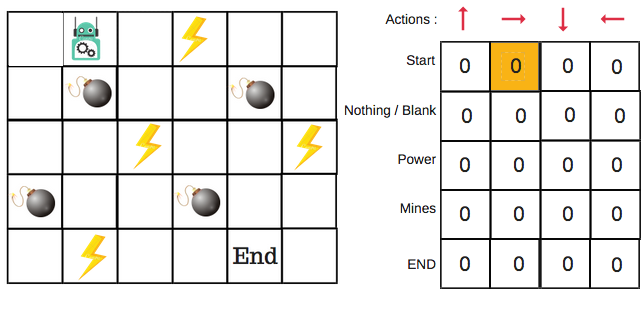
\includegraphics[scale=0.5]{pix/q_learning/q_robot_maze_perform_action.png}
\caption{Maze: perform an action}
%\label{fig:label}
\end{figure}

We can now update the $Q$-values for being at the start and moving right using the 
Bellman equation.


\subsubsection{Steps 4 and 5: evaluate}

Now we have taken an action and observed an outcome and reward. We need to update 
the function $Q(s,a)$.

\begin{figure}[!htb]
\centering
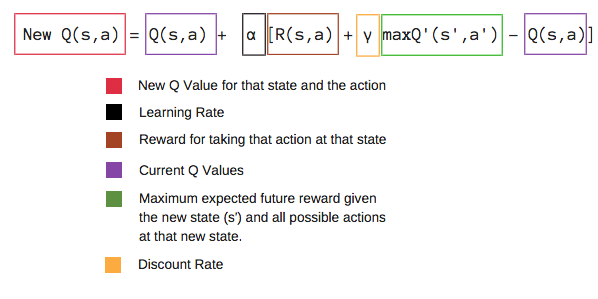
\includegraphics[scale=0.5]{pix/q_learning/q_robot_maze_q_function.png}
\caption{Maze: q-function}
%\label{fig:label}
\end{figure}

In the case of the robot game, to reiterate the scoring/reward structure is:

\begin{itemize}
%\setlength{\itemsep}{0pt}
%\setlength{\parsep}{0pt}
\setlength{\parskip}{0pt}
\item[-]
power $= +1$
\item[-]
mine $= -100$
\item[-]
end $= +100$
\end{itemize}

\begin{figure}[!htb]
\centering
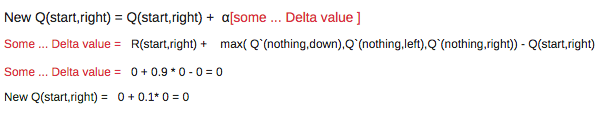
\includegraphics[scale=0.7]{pix/q_learning/q_robot_maze_iteration.png}
%\caption{Maze: q-function}
%\label{fig:label}
\end{figure}
We will repeat this again and again until the learning is stopped. In this way 
the $Q$-Table will be updated.


\section{Implementation using python}


